\subsection{Application Installation} \label{subsection:android-install}
Before running an application, the \gls{apk} containing the code, has to be installed.
The installation consists of two major steps.
The first step is primarily about verification, while the second step is the bytecode optimization and, in case of \gls{art}, the code compilation (see figure~\ref{fig:install}).
The differences will be explained in the following subsections.
\newline
The \textit{META-INF} folder contains the necessary files for performing the signature verification process.
The three files are the \textit{MANIFEST.MF}, the \textit{MANIFEST.SF} und the \textit{CERT.RSA}.
The \textit{CERT.RSA} contains the public key to decrypt the \textit{MANIFEST.SF} and compare it to the \textit{MANIFEST.MF}.
The manifest \textit{MANIFEST.MF} contains the complete list of files and their signatures of the \gls{apk}, e.g. \textit{classes.dex}.
While the manifest files are used to detect tampering, the certificate is used to identify the code signer but as said before only in an abstract way that cannot be linked to a real world entity.
Since Android allows self-signed certificates, there is no authority defining right or wrong, e.g. if an application is authentic or a signing developer is a pirate. \cite{codeSigning} \cite{androidSigning} \cite{nelenkovSelf}
\newline
The installation can be performed in two ways depending on the runtime of the Android \gls{os}.
For the \gls{dvm}, optimisation is applied to the \textit{classes.dex} file and the corresponding \gls{odex} file is generated and moved to the Dalvik cache.
As a reminder, an \gls{odex} file is an optimization tailored for optimal performance on a specific device performed on installation.
\newline
Currently, the Android runtime of choice is \gls{art}.
For this runtime, the second step is more complex, since the bytecode has to be compiled an additional time.
This will be explained in section~\ref{subsection:android-art}.
\newline
\begin{figure}[h]
    \centering
    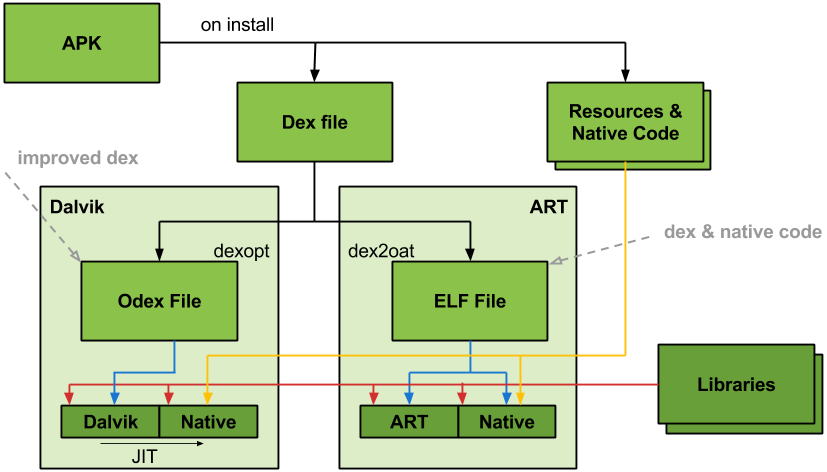
\includegraphics[width=0.8\textwidth]{data/install.png}
    \caption{Installing an \gls{apk} on a device \cite{googleIOArt}}
    \label{fig:install}
\end{figure}
\newline
After the bytecode is optimized respectively compiled, the application can be run.
When run on the device, Android creates a sandboxed environment for this application only.
